\documentclass[10pt,a4paper]{report}


\usepackage{amsmath}
\usepackage[utf8]{inputenc}
\usepackage{amsmath}
\usepackage{amsfonts}
\usepackage{amssymb}
\usepackage{calrsfs}
\usepackage[left=2cm,right=2cm,top=2cm,bottom=2cm]{geometry}
\usepackage[mathscr]{euscript}
\usepackage{mathrsfs}

%%%%%%%%%for adding margins%%%%%%%%%
\usepackage{scrextend}
%%%%%%%%%%%%%%%%%%%%%%%%%%%%%%%

%for drawing commutative diagrams.
\usepackage{tikz-cd}  
%%%%%%%%%%%%%%%%%%%%%%%%%%%


%%%%%%%%%%%for wide hat%%%%%%%%%%%%
\usepackage{scalerel,stackengine}
\stackMath
\newcommand\reallywidehat[1]{%
\savestack{\tmpbox}{\stretchto{%
  \scaleto{%
    \scalerel*[\widthof{\ensuremath{#1}}]{\kern-.6pt\bigwedge\kern-.6pt}%
    {\rule[-\textheight/2]{1ex}{\textheight}}%WIDTH-LIMITED BIG WEDGE
  }{\textheight}% 
}{0.5ex}}%
\stackon[1pt]{#1}{\tmpbox}%
}

%\renewcommand{\hat}{\reallywidehat}
%%%%%%%%%%%%%%%%%%%%%%%%%%%%%%%%%%
\renewcommand{\hat}{\widehat}


%%%%%%%%%%for changing margin
\def\changemargin#1#2{\list{}{\rightmargin#2\leftmargin#1}\item[]}
\let\endchangemargin=\endlist 

\newenvironment{proof}
{\begin{changemargin}{1cm}{0.5cm}
	}%your text here
	{\end{changemargin}
}
\newenvironment{subproof}
{\begin{changemargin}{0.5cm}{0.5cm}
	}%your text here
	{\end{changemargin}
}
%%%%%%%%%%%%%%%%%%%%%%%%%%%%%

\usepackage{empheq}
%%%%%%%%%%for writing symbol above an equality
\newcommand{\xeq}[1]{\stackrel{\mathclap{\normalfont\mbox{\tiny{#1}}}}{=}}
%%%%%%%%%%%%%%%%%%%%%%%%%%%%%%%%%%%%%%%%%%%%

\begin{document}
\newcommand{\thm}{\textbf{Theorem) }}
\newcommand{\thmnum}[1]{\textbf{Theorem #1) }}
\newcommand{\defi}{\textbf{Definition) }}
\newcommand{\lem}{\textbf{Lemma) }}
\newcommand{\lemnum}[1]{\textbf{Lemma #1) }}
\newcommand{\prop}{\textbf{Proposition) }}
\newcommand{\propnum}[1]{\textbf{Proposition #1) }}
\newcommand{\cor}{\textbf{Corollary) }}
\newcommand{\cornum}[1]{\textbf{Corollary #1) }}


\newcommand{\pf}{\textbf{proof) }}
\newcommand{\eop}{\hfill  \textsl{(End of proof)} $\square$} %end of proof


\newcommand{\lap}{\triangle} %%Laplacian
\newcommand{\s}{\vspace{10pt}}
\newcommand{\bull}{$\bullet$}
\newcommand{\sta}{$\star$}
\newcommand{\reals}{\mathbb{R}}

\newcommand{\intN}{\mathbb{Z}_N}
\newcommand{\norms}[2]{\parallel #1 \parallel_{#2}}
\newcommand{\avg}{\mathbb{E}}
\newcommand{\prob}{\mathbb{P}}
\newcommand{\osc}{\text{\osc}}

\newcommand{\boxinn}[4]{\begin{array}{|cc|} 
\cline{1-2}
#1 & #2 \\
#3 & #4 \\
\cline{1-2}
\end{array}}

\newcommand{\newday}{================================================================}
\newcommand{\digression}{**********************************************************************************************}

\renewcommand{\bar}{\overline}

\setlength\parindent{0pt}

\chapter*{Introduction to Discrete Analysis}
\s

Lecturer : Prof. Tim Gowers
\s

\newday

(4th October 2018, Thursday)
\s

\section*{Chapter 1. The discrete Fourier transform}
\s

Let $N$ be some fixed positive integer. Write $\omega$ for $e^{2\pi i /N}$. and $\mathbb{Z}_N$ for $\mathbb{Z}/N\mathbb{Z}$. Let $f: \mathbb{Z}_N \rightarrow \mathbb{C}$. Given $r \in \mathbb{Z}_N$ define $\hat{f}(r)$ to be $\frac{1}{N} \sum_{x \in \mathbb{Z}_N} f(x) \omega^{-rx}$. From now on, we shall use the notation $\mathbb{E}_{x\in \mathbb{Z}_N}$ for $\frac{1}{N} \sum_{x \in \mathbb{Z}_N}$(so that $\hat{f}(r)  = \mathbb{E}_x f(x)e^{-2\pi i rx/N}$). If we write $\omega_r$ for the function $x\mapsto \omega^{rx}$ and $\langle f,g \rangle$ for $\mathbb{E}_x f(x)\bar{g(x)}$, then $\hat{f}(r) = \langle f,\omega_r \rangle$.
\s

Let us write $\norms{f}{p}$ for $(\mathbb{E}_x |f(x)|^p)^{1/p}$ and call the resulting space $L_p(\mathbb{Z}_N)$.
\s

\textbf{Important convention} : we use averages for the "original functions" in "physical space" and sums for their Fourier transforms in "frequency spaces".
\s

\lemnum{1} (Parseval's identity) If $f,g:\mathbb{Z}_N \rightarrow \mathbb{C}$, then $\langle \hat{f},\hat{g}\rangle =\langle f,g\rangle$.
\begin{itemize}
\item[ ] \pf
\begin{align*}
\langle \hat{f},\hat{g} \rangle &= \sum_{r} \hat{f}(r) \bar{\hat{g}(r)} = \sum_r (\mathbb{E}_x f(x)\omega^{-rx} \bar{(\mathbb{E}_y g(y) \omega^{-ry})} ) \\
&= \mathbb{E}_x \mathbb{E}_y f(x)\bar{g(y)} \sum_r \omega^{-r(x-y)} \\
&= \mathbb{E}_x \mathbb{E}_y f(x)\bar{g(y)} \Delta_{xy}\\
&=  \mathbb{E}_x f(x) \mathbb{E}_y \bar{g(y)} \Delta_{xy} = \mathbb{E}_x f(x)\bar{g(x)} = \langle f,g \rangle
\end{align*}

where $\Delta_{xy} = N$ if $x=y$ and $0$ if $x\neq y$.(in analogy with $\delta$-distribution).

\eop
\end{itemize}
\s

Beware that inner product in the Fourier space and the physical space are defined in a different way : $\langle \hat{f},\hat{g} \rangle = \sum_{r} \hat{f}(r) \bar{\hat{g}(r)}$ while $\langle f,g\rangle = \avg_x f(x) \bar{g}(x)$
\s

\lemnum{2}(Convolution identity) $\hat{f * g}(r) = \hat{f}(r) \hat{g}(r)$

\begin{itemize}
\item[ ]\pf The convolution $f*g(x)$ is defined to be $\avg_{y+z =x} f(y) g(z) = \avg_y f(y)g(x-y)$. Then,
\begin{align*}
\hat{f * g}(r) &= \avg_x f*g(x) \omega^{-rx} = \avg_x \avg_{y+z =x} f(y) g(z) \omega^{-rx} \\
&= \avg_x \avg_{y+z=x} f(y) g(z) \omega^{-ry}\omega^{-rz} = \avg_y f(y) \omega^{-ry} \avg_{z} g(z) \omega^{-rz} = \hat{f}(r) \hat{g}(r)
\end{align*}
\eop
\end{itemize} 
\s

\lemnum{3}(Inversion formula)  $f(x) = \sum_{r} \hat{f}(r)\omega^{rx}$.
\begin{itemize}
\item[ ] \pf
\begin{align*}
\sum_{r} \hat{f}(r) \omega^{rx} = \sum_r \avg_y f(y) \omega^{r(x-y)} = \avg_y f(y) \sum_r \omega^{r(x-y)} = \avg_y f(y) \Delta_{xy}  = f(x)
\end{align*}
\eop

\end{itemize}
\s

\textbf{Further Observations} :

\begin{itemize}
\item If $f$ is real-valued, then $\hat{f}(-r) = \avg_x f(x) \omega^{rx} = \bar{\avg_x f(x) \omega^{-rx}} = \overline{ \hat{f}(r) }$.

\item If $A\subset \intN$, write $A$(instead of $1_A$ or $\chi_A$) for the characteristic function of $A$. Then $\hat{A}(0) = \avg_x A(x) = \frac{|A|}{N}$, the \textbf{density} of $A$. Also, $\norms{\hat{A}}{2}^2 = \langle \hat{A}, \hat{A} \rangle = \langle A,A \rangle = \avg_x A(x)^2 = |A|/N$.

\item Let $f: \intN \rightarrow \mathbb{C}$. Given $\mu \in \intN$ with $(\mu, N)=1$, define $f_{\mu}(x)$ to be $f(\mu^{-1}x)$. Then $\hat{f}_{\mu}(r) = \avg_x f_{\mu}(x)\omega^{-rx} = \avg_x f(x/\mu) \omega^{-rx} = \avg_x f(x)\omega^{-r\mu x} = \hat{f}(\mu r)$.
\end{itemize}

\subsection*{Roth's Theorem}
\s

\thmnum{4}(Szemer\'{e}di's theorem for $k=3$) For every $\delta >0$, there exists $N$ such that if $A \subset \{1, \cdots, N\}$ is a set of size at least $\delta N$, then $A$ must contain an arithmetic progression of length 3. 

\s

Basic strategy : show that if $A$ has density $\geq \delta$ and no 3AP, then there is a long arithmetic progression $P \subset \{1,\cdots,n\}$ such that
\begin{align*}
|A\cap P| \geq (\delta + c(\delta)) |P|
\end{align*}

====================================================================================
(9th October, Tuesday)
\s

\thmnum{4}(Roth's theorem, or Szemer\'{e}di's theorem for $k=3$) For every $\delta >0$, there exists $N$ such that if $A \subset \{1, \cdots, N\}$ is a set of size at least $\delta N$, then $A$ must contain an arithmetic progression of length 3. 
\s

\lemnum{5} Let $A,B,C \subset \intN$ have densities $\alpha,\beta,\gamma$. If $\max_{r\neq 0} |\hat{A}(r)| \leq \frac{\alpha(\beta \gamma)^{1/2}}{2}$ and $\frac{\alpha \beta \gamma}{2} > \frac{1}{N}$ then there exist $x, d \in \intN$ with $d\neq 0$ s.t. $(x,x+d,x+2d) \in A \times B \times C$.
\begin{proof}
\pf Assume $N$ is odd.

Consider the function $A(x)B(x+d)C(x+2d)$, which is non-zero if and only if there is a arithmetic progression of length 3. So $\avg_{x,d} A(x)B(x+d)C(x+2d)$ counts the density of $x,d$ satisfying such condition.
\begin{align*}
& \avg_{x,d}A(x)B(x+d)C(x+2d) = \avg_{x+z =2y}A(x)B(y)C(z) \\
=& \avg_{u}\big( \avg_{x+z =u} A(x)C(z) \big) \avg_{2y=u} B(y) = \avg_u A * C(u) B_2(u) = \langle A * C, B_2 \rangle \\
=& \langle \hat{A*C}, \hat{B}_2 \rangle = \langle \hat{A} \hat{C}, \hat{B}_2 \rangle = \sum_r \hat{A}(r) \hat{C}(r) \hat{B}(-2r) \\
=& \alpha \beta \gamma + \sum_{r\neq 0} \hat{A}(r) \hat{C}(r) \hat{B}(-2r)
\end{align*}
\textit{(Recall, $B_{\mu}(x)$ is defined to be $B(\mu^{-1}x)$ whenever $(\mu, N)=1$. We can generalize this to write $B_{\mu}(x) = \avg_{\mu u=x}B(u)$  )}

The first term $\alpha \beta \gamma$ gives a rough estimate of the value just in terms of the densities and the second term gives an estimate for how random the sets $A,B,C$ behave.
\begin{align*}
\big|\sum_{r\neq 0} \hat{A}(r) \hat{B}(-2r) \hat{C}(r) \big| &\leq \frac{\alpha (\beta \gamma)^{1/2}}{2} \sum_{r\neq 0} \big|\hat{B}(-2r)\big| \big|\hat{C}(r)\big| \\
&\leq \frac{\alpha (\beta \gamma)^{1/2}}{2} \big( \sum_r \big| \hat{B}(-2r) \big|^2 \big)^{1/2} \big( \sum_r \big| \hat{C}(r) \big|^2 \big)^{1/2} \quad \text{(Cauchy-Schwarz)} \\
& = \frac{\alpha (\beta \gamma)^{1/2}}{2} \norms{\hat{B}}{2} \norms{\hat{C}}{2} = \frac{\alpha (\beta \gamma)^{1/2}}{2} \norms{B}{2} \norms{C}{2} \quad \text{(Parseval)} \\
& = \frac{\alpha \beta \gamma}{2}
\end{align*}
The contribution to $\avg_{x,d}A(x)B(x+d)C(x+2d)$ from $d=0$ is at most $\frac{1}{N}$, so if $\frac{\alpha \beta \gamma}{2} > \frac{1}{N}$, we are done.

\eop
\end{proof}
\s

Now let $A$ be a subset of $\intN$ of density $\geq \delta$ and let $B=C = A\cap [\frac{N}{3},\frac{2N}{3}]$. 

\begin{itemize}
\item  If $B$ has density $< \frac{\delta}{5}$, then either $A \cap [1,\frac{N}{3}]$ or $A\cap [\frac{2N}{3},N]$ has density at least $\frac{2\delta}{5}$ so in that case we find an AP(arithmetic progression), $P$(one of $\intN \cap [1,N/3]$ and $\intN \cap [2N/3,N]$), of length about $N/3$ such that $|A\cap P| /|P| \geq 6\delta /5$.

\item Otherwise, if $\max_{r\neq 0} |\hat{A}(r)| \leq \frac{\delta^2}{10}$. We may pick $N$ large so that $\frac{\delta^3}{50} > \frac{1}{N}$. Then $A \times B \times C$ contains a 3AP by the \textbf{Lemma 5} and therefore $A$ contains a 3AP.

\item So if $A$ does not contain a 3AP, then either we find $P$ of length about $N/3$ with $|A \cap P|/|P| \geq 6\delta/5$ or we find $r\neq 0$ such that $|\hat{A}(r)| \geq \delta^2/10$. (This is sometimes called the \emph{dichotomy of order and chaos})
\end{itemize}

\s

\defi If $X$ is a finite set and $f: X \rightarrow \mathbb{C}$, $Y\subset X$, write $\text{osc}(f\big|_{Y})$ to mean $\max_{y_1,y_2 \in Y} |f(y_1) - f(y_2) |$.
\s

\lemnum{6} Let $r \in \hat{\mathbb{Z}}_N$(or just $\intN$) and let $\epsilon>0$. Then there is a partition of $\{ 1,2,\cdots, N\}$ into arithmetic progressions $P_i$ of length at least $c(\epsilon)\sqrt{N}$ such that $\text{osc}(\omega_r \big|_{P_i}) \leq \epsilon$ for each $i$.

\begin{proof}
\pf Let $t= \lfloor \sqrt{N} \rfloor$. Of the numbers $1,\omega^r,\cdots,\omega^{tr}$ there must be two that differ by at most $2\pi/t$(by sort-of-pigeon hole principle.) If $|\omega^{ar} - \omega^{br} | \leq 2\pi /t$ with $a<b$, then $|1-\omega^{dr}| \leq 2\pi /t$ where $d= b-a$. Now, by the triangular inequality, if $u<v$ then
\begin{align*}
|\omega^{urd} - \omega^{vrd} | \leq |\omega^{urd} - \omega^{(u+1)rd} | + \cdots + |\omega^{(v-1)rd} - \omega^{vrd} | \leq \frac{2\pi}{t} (v-u)
\end{align*}
So if $P$ is a progression with common difference $d$ and length $l$, then $\text{osc} (\omega_{r} \big|_{P}) \leq \frac{2\pi l}{t}$. So divide up $\{1,\cdots, N\}$ into residue classes root $d$ and partition each residue class into parts of length between $\frac{\epsilon t}{4\pi}$ and $\frac{\epsilon t}{2\pi}$(this is possible, since $d\leq t \leq \sqrt{N}$.) We are done, with $c(\epsilon) = \frac{\epsilon}{16}(<\frac{\epsilon}{4\pi})$.

\eop
\end{proof}
\s

Now let us use the  information that $r\neq 0$ and $|\hat{A}(r) | \geq \delta^2/10$.

Define the \textbf{balanced function} $f$ of $A$ by $f(x) = A(x) - |A|/N$ for each $x$. Note that $\hat{f}(0) =0 $ and $\hat{f}(r) = \hat{A}(r)$ for all $r\neq 0$.

Now let $P_1, \cdots, P_m$ be given by \textbf{Lemma 6} with $\epsilon = \delta^2/20$. Then
\begin{align*}
\frac{\delta^2}{10} &\leq |\hat{f}(r)| = \frac{1}{N} \big| \sum_x f(x) \omega^{-rx} \big| \leq \frac{1}{N} \sum_i \big| \sum_{x\in P_i}  f(x) \omega^{-rx} \big | \\
&\leq \frac{1}{N} \sum_{i=1}^m \Big[ \big| \sum_{x\in P_i} f(x) \omega^{-rx_i} \big| + \big| \sum_{x\in P_i} f(x)(\omega^{-rx} - \omega^{-rx_i})   \big|     \Big] \quad \text{where } x_i \text{ arbitrary} \in P_i \\
&\leq \frac{1}{N} \sum_{i=1}^N \big| \sum_{x\in P_i} f(x) \big| + \frac{\delta^2}{20}
\end{align*}
So $\sum_{i=1}^n \big| \sum_{x_i\in P_i} f(x) \big| \geq \delta^2 N/20$. Also, $\sum_{i=1}^m \sum_{x\in P_i} f(x) =0$. So
\begin{align*}
\sum_{i=1}^m \Big(  \big| \sum_{x\in P_i} f(x) \big| + \sum_{x\in P_i}f(x) \Big) \geq \frac{\delta^2}{20} \sum_{i=1}^m |P_i|
\end{align*}
Therefore, $\exists i$ s.t. $|\sum_{x\in P_i} f(x) | + \sum_{x\in P_i}f(x) \geq \frac{\delta^2}{20} |P_i|$ by pigeon hole principle and hence $\sum_{x\in P_i}f(x) \geq \frac{\delta^2}{40}|P_i|$. This implies $|A\cap P_i | = \big| \sum_{x\in P_i} f(x) + \frac{|A|}{N}  \big|   \geq (\delta + \delta^2/40)|P_i|$
\s

\newday

(11th October, 2018)
\s

(Example sheets handed out - do not try to use particular theorem, but to apply the idea of using Fourier analysis in combinatorics.

Why does Fourier analysis have anything to do with combinatorics? Because we can formulate various problems in terms of Fourier transformation, e.g. by convolution and Parseval's law.)
\s

\bull What we have showed : Let $A \subset \intN$, $|A|\geq \delta N$. Then,
\begin{itemize}
\item[(1)] $A$ contains a 3AP \emph{or}
\item[(2)] $N$ is even \emph{or}
\item[(3)] $\exists P \subset \{ 1,\cdots, N\}$, $|P|\geq N/3$ s.t. $|A\cap P| \geq \frac{6\delta}{5} |P|$ \emph{or}
\item[(4)] $\exists P \subset \{1,\cdots, N\}$, $|P| \geq \frac{\delta^2}{320} \sqrt{N}$ s.t $|A\cap P| \geq (\delta + \delta^2/40)|P|$
\end{itemize}

\quad If (2) holds, write $N=N_1+N_2$ with $N_1, N_2$ odd, $N_1, N_2 \simeq N/2$. Then $A$ has density at least $\delta$ in one of $\{1,\cdots, N_1\}$ or $\{N_1 +1, \cdots, N_1 + N_2\}$.

\quad If (4) holds (NB (3)$\Rightarrow$ (4)) then we pass to $P$ and start again(that is, replace $\intN$ with $P$ and $A$ with $A\cap P$). After $40/\delta$ iterations, the density at least doubles. So the total number of iterations we can have is at most $\leq \frac{40}{\delta} + \frac{40}{2\delta} + \frac{40}{4\delta} + \cdots \leq \frac{80}{\delta}$.

\quad If $\frac{\delta^2}{320} \sqrt{N} \geq N^{1/3}$ at each iteration, and $\delta^3/25 \geq N^{-1}$ (which follow from the first condition) then after $\frac{80}{\delta}$ iterations, we have is $N\geq N^{(1/3)^{80/\delta}}$. So the argument works provided
\begin{align*}
&N^{(1/3)^{80/\delta}} \geq \Big( \frac{320}{\delta^2} \Big)^6 \Leftrightarrow \Big( \frac{1}{3} \Big)^{80/\delta} \log N \geq 6(\log 320 + 2\log \frac{1}{\delta}) \\
\Leftrightarrow \quad & \frac{-80}{\delta} \log 3 + \log \log N \geq \log 6 + \log (\log 320 + 2\log \frac{1}{\delta}) \\
\Leftarrow \quad &\log \log N \geq \frac{160}{\delta} \\
\Leftarrow \quad &\delta\geq \frac{160}{\log \log N}
\end{align*}
(just the follow the idea of calculation,,, do not try to learn a particular thing from this calculation)

(In fact 320 above should be corrected to 640 because of (2))
\s

\subsection*{Bogolyubov's Method}

\defi Let $K \subset \hat{\mathbb{Z}}_N$ and let $\delta >0$. The \textbf{Bohr set} $B(K,\delta)$ has two definitions.
\begin{itemize}
\item[(1)] $B(K,\delta) = \{x\in \intN : rx \in [-\delta N, \delta N] \quad \forall r\in K \}$ (arc-length definition)
\item[(2)] $B(K,\delta) = \{x\in \intN : |1- \omega^{rx}| \leq \delta \quad \forall r\in K|\}$ (chord-length definition)
\end{itemize}
\s

It turns out that Bohr set has a lot of structure.
\s

\defi Let $G$ be an Abelian group and let $A,B$ be subsets of $G$. Then 
\begin{align*}
A+B = \{ a+b: a\in A, b\in B\} \\
A-B = \{a-b: a\in A, b\in B\} \\
rA = \{a_1+ \cdots + a_r : a_1,\cdots,a_r \in A  \}
\end{align*}
\s

\lemnum{7} \emph{(Bogolyubov)} Let $A\subset \intN$ be a set of density $\alpha$. Then $2A-2A$ contains a Bohr set $B(K,1/4)$(arc) with $|K|\leq \alpha^{-2}$.

\begin{proof}
\pf Observe that $x\in 2A-2A$ if and only if $A*A*(-A)*(-A)(x) \neq 0$(think for a second). But
\begin{align*}
A*A*(-A)*(-A)(x) &= \sum_{r} \reallywidehat{A*A*(-A)*(-A)}(r) \omega^{rx} \quad \text{(inversion formula)} \\
&= \sum_r  \big| \hat{A}(r) \big|^4 \omega^{rx}
\end{align*}
Let $K = \{r: \big| \hat{A}(r) \big| \geq \alpha^{3/2} \}$. Then 
\begin{align*}
\alpha = \norms{\hat{A}}{2}^2 = \sum_{r} \big| \hat{A}^2(r) \big|^2 \geq \alpha^3 |K|
\end{align*}
so $|K| \leq \alpha^{-2}$.
\quad Now suppose that $x\in B(K,1/4)$. Then 

\begin{align*}
\sum_{r} \big| \hat{A}(r)\big|^4 \omega^{rx}  = \alpha^4 + \sum_{r\in K,r\neq 0} \big| \hat{A}(r)\big|^4 \omega^{rx} + \sum_{r \notin K} \big| \hat{A}(r)\big|^4 \omega^{rx}
\end{align*}
The real part of the second term is non-negative, since $rx\in [-N/4,N/4]$ when $r\in K$. Also the final term can be bounded by
\begin{align*}
\Big| \sum_{r \notin K} \big| \hat{A}(r)\big|^4 \omega^{rx} \Big| \leq \sum_{r \notin K} \big| \hat{A}(r)\big|^4 < \alpha^3 \sum_{r \notin K} \big| \hat{A}(r)\big|^2 \leq \alpha^4
\end{align*}
It follows that $\text{Re}\Big( \sum_r  \big| \hat{A}(r) \big|^4 \omega^{rx} \Big) >0$, so $x\in 2A-2A$.

\eop
\end{proof}
\s

\lemnum{8} Let $K \subset \intN$ and let $\delta >0$. Then
\begin{itemize}
\item[(i)] $B(K,\delta)$ has density at least $\delta^{|K|}$.
\item[(ii)] $B(K,\delta)$ contains a mod-$N$ arithmetic progression of length $\geq \delta N^{1/|K|}$.
\end{itemize}
\begin{proof}
\pf

\begin{itemize}
\item[(i)]Let $K = \{r_1,\cdots, r_k\}$. Consider the $N$ number of $k$-tuples $(r_1 x, \cdots, r_k x)\in \intN^k$(for $x\in \intN$). If we intersect this set of $k-tuples$ with a random "box" $Q=[t_1,t_1+\delta N] \times \cdots \times [t_k,t_k+\delta N]$. Then the expected number of $k$-tuples in the box is $\delta^k N$(since each intersection has probability $\delta^k$.)

\quad But if $(r_1 x,\cdots, r_k x)$  and $(r_1 y,\cdots, r_k y)$ belong to this box, then $x-y \in B(K,\delta)$, so the expected number of in $(r_1 y,\cdots, r_k y)$ is smaller or equal to the expected number of $y$ in $B(K,\delta)$. i.e. if we let $q$ be a random point in $Q \cap \intN^k$, then
\begin{align*}
\avg( \sum_y 1_{y\in B(K,\delta)}) \geq \avg(\sum_{y} 1_{q \in Q} 1_{q + y  \in Q}) = \sum_y \prob ( y\in Q  ) = N |\delta|^{K}
\end{align*}
(there must be an easy argument... in fact, in the lecture, it was concluded before ~so the expected number of, so there must be more intuitive way of understanding this)
\item[(ii)] If we take $\eta > N^{-1/k}$, then by (i) we get that $|B(K,\eta)|>1$ so $\exists x \in B(K,\eta)$ s.t. $x\neq 0$. But then $dx \in B(K,d\eta)$ for every $d$. So if $d\eta \leq \delta$ then $B(K,d\eta) \subset B(K,\delta)$ so $dx\in B(K,\delta)$, that gives us an AP of length at least $\delta/\eta$. So we get one of length at least $\delta N^{1/k}$.
\end{itemize} 
\eop
\end{proof}
\s

\newday

(16th October, Tuesday)
\s

(about the example sheet - Question 2, has to fix $\alpha^2 \beta^2 N^4$ to $\alpha^2 \beta^2 N^3$ : a natural way to think about this is "normalizing". We decide one element from other three, so the factor of $N$ should be 3.)
\s

Recall : $B(K,\delta) = \{x\in \intN : rx\in [-\delta N, \delta N]$ for all $r\in K \}$
\s

\defi Let $A$, $B$ be subsets of Abelian groups and let $\phi : A\rightarrow B$. Then $\phi$ is a \textbf{Freiman homomorphism of order $k$} if
\begin{align*}
a_1 + \cdots + a_k = a_{k+1} + \cdots + a_{2k} \quad \Rightarrow \quad \phi(a_1) + \cdots \phi(a_k) = \phi(a_{k+1}) +\cdots +\phi(a_{2k})
\end{align*}
If $k=2$, we call this a \textbf{Freiman homomorphism}. In that case, the condition is equivalent to
\begin{align*}
a-b = c-d \quad \Rightarrow \quad \phi(a) - \phi(b) = \phi(c) - \phi(d)
\end{align*}

\quad If $\phi$ has an inverse which is also a Freiman homomorphism of order $k$ then $\phi$ is a \textbf{Freiman isomorphism of order $k$}.


\s

Consider \quad $\begin{matrix}
\cdot & \cdot & \cdot \\
\cdot & \cdot & \cdot \\
\cdot & \cdot & \cdot
\end{matrix}
$ \quad and $\cdots$, $\cdots$, $\cdots$. They have same additive structure, in some sense, and the Freiman isomorphism describes this. Freiman isomorphism is intended to describe a hidden lattice structure of a additive system.
\s

\renewcommand{\vec}{\underline}

\lemnum{9} Assume $0 \notin K$ and $N$ prime. If $\delta <1/4$, then $B(K,\delta)$ (arc) is Freiman isomorphic to the intersection $[-\delta N, \delta N]^{|K|} \cap \Lambda \subset \reals^{|K|}$ where $\Lambda$ is some lattice in $\reals^{|K|}$. 
\begin{proof}
\pf Let $K = \{r_1, \cdots, r_k\}$ and let $\Lambda = N \mathbb{Z}^k + \{(r_1x, \cdots, r_kx) : x\in \mathbb{Z}\}$. Write $\vec{r}$ for $(r_1, \cdots, r_k)$. \emph{Claim} that $B(K,\delta) \cong\Lambda \cap [-\delta N, \delta N]^k$.
\s

\quad Define a map $\phi : B(K,\delta) \rightarrow \Lambda \cap [-\delta N,\delta N]^k$ by
\begin{align*}
x \mapsto (\langle r_1 x\rangle, \cdots, \langle r_k x\rangle)
\end{align*}
where $\langle u\rangle$ means the least-modulus residue of $u$ mod $N$. If $x+ y = z+w$, then $\vec{r} x+ \vec{x} y = \vec{r} z + \vec{r} w$ in $\intN^k$. But for each $i$, $\langle r_i x \rangle + \langle r_i y \rangle - \langle r_i z \rangle- \langle r_i w \rangle \in [-4\delta N, 4\delta N]$. Since $\delta < 1/4$, that implies that $\langle r_i x \rangle + \langle r_i y \rangle - \langle r_z \rangle- \langle r_i w \rangle =0$. So $\langle \vec{r} x \rangle + \langle \vec{r} y \rangle - \langle \vec{r} \rangle- \langle \vec{r} w \rangle = \vec{0}$.

\quad That already implies that $\phi$ is an injection.

\quad If $\vec{r} x + \vec{a} N \in [-\delta N, \delta N]^k$(this is a way of writing a typical point in a lattice), then $r_i x \in [-\delta N, \delta N]$ mod $N$ for each $i$, so $x\in B(K,\delta)$ and $\phi(x) = \vec{r}x + \vec{a}N$. So $\phi$ is a surjection.

\quad If $\vec{r} x+ \vec{a} N + \vec{r} y + \vec{b} N = \vec{r} z + \vec{c}N + \vec{ r} w + \vec{d}N$, then $r_i(x+y) = r_i (z+w)$ mod $N$, s $x+y = z+w$ mod $N$, so the inverse of $\phi$ is also a Freiman homomorphism.

\eop 
\end{proof}
\s

(we will not prove in this course, but later in next term, we will prove a generalized version of AP contained in an intersection of $K$ and a box - this requires more knowledge in geometry of numbers, so cannot be dealt here)
\s

\lemnum{10} Let $\Lambda$ be a lattice and let $C$ be a symmetric convex body, both in $\reals^k$. Then $|\Lambda \cap C | \leq 5^k |\Lambda \cap \frac{C}{2}|$

(5 is not an optimal bound, but convenient to prove - how do we reduce this?)
\begin{proof}
\pf Let $x_1, \cdots, x_n$ be a maximal subset of $\Lambda \cap C$ such that for all $i \neq j$, $x_j \notin x_i + \frac{C}{2}$. Then by maximality, the sets $x_i + C/2$ cover all of $\Lambda \cap C$. So we see that
\begin{align*}
|A \cap C|  = \big| \cup_i (x_i + C/2) \cap A \big| \leq n \big|A \cap C/2 \big|
\end{align*}
Also, the sets $x_i + C/4$ are disjoint subsets of $\reals^k$, and they are all contained in $C + \frac{C}{4} = 5C/4$. That is $\cup_i (x_i + C/4) \subset 5C/4$ and therefore
\begin{align*}
\big| \cup_i (x_i + C/4) \big| = n \big| C/4 \big| \leq \big| 5C/4 \big|
\end{align*}
Hence $n \leq \frac{\text{vol}(5C/4)}{\text{vol}(C/4)} = 5^k$, and we have the conclusion along with the previous inequality.
\end{proof}
\s

\cornum{11} If $N$ is primes, $0\notin K$, $|K| =k$, $\delta <1/4$, then $|B(K,\delta)| \delta 5^k |B(k,\delta/2)|$
\s

\section*{2. Sum Sets and their Structure}

Suppose $A$ is a subset of integers, and has $k$ such that $|A+A | \leq k|A|$. What can we say about the set $A$? What can we say about the bound of $|rA-sA|$? (will prove $|rA-sA| \leq k^{r+s}|A|$)
\s

\lemnum{1} (George Petridis - a former student of T.W.Gowers) Let $A_0$ and $B$ be finite subsets of an Abelian group such that $|A_0 + B | \leq K_0 |A_0| $. Then there exists a subset $A\subset A_0$ and $K\leq K_0$ such that $|A+B+C|\leq K|A+C|$ for every finite subset $C$ of the group.
\s

-the style of proof is so different from other combinatorics proofs. It uses induction on $C$.(Lesson to take : do not dispose a method for proof even before thinking about it)
\begin{proof}
\pf Choose $A \subset A_0$ that minimizes the ratio $|A+B|/|A|$ and let the minimal ratio be $K$.

\begin{subproof}
$\star$ Claim : This particular choice of $A$ and $K$ works - We prove this by induction on $C$.

\pf If $C=\phi$, we are all happy.

Now assume it for $C$ and let $x\notin C$. Then $A+(C \cup \{x\}) = (A+C) \cup \Big[ (A+x) \backslash (A'+x) \Big]$ where $A' = \{a\in A: a+x\in A+ C\}$. This is a disjoint union, so
\begin{align*}
|A+(C\cup \{x\})| = |A+C| + |A| - |A'|
\end{align*}
Also, $A+B + (C\cup \{x\}) = (A+B+C) \cup \big( (A+B+x) \backslash (A'+B+x)\big)$ since if $a+x\in A+C$, then $a+B+x \subset A+B+C$.
\begin{align*}
|A+B+(C\cup \{x \}) | &\leq |A+B+C| + |A+B| - |A'+B| \\
&\leq K|A+C| + K|A| - K|A'| \\
& = |A+(C\cup \{x\})|
\end{align*}
by induction and minimality property of $A$
\end{subproof}

\eop
\end{proof}
\s

\newday

(18th October, Thursday)
\s

(Example class next Wednesday afternoon, 24th October)
\s

\cornum{2} If $A$, $B$ are finite subsets of an Abelian group and $|A+ B|\leq K|A|$ then there exists $A' \subset A$, $A' \neq \phi$ such that $|A' + rB| \leq K^r|A'|$ for every positive integer $r$.
\begin{proof}
\pf Choose $A'$ as we chose $A$ in \textbf{Lemma 1}, that is, minimizing $|A'+B|/|A'|$. Then $|A' + rB| = |A'+B +(r-1)B| \leq K |A' + (r-1)B|$ and $|K' + B| \leq K|A'|$. So we are done by induction.

\eop
\end{proof}
\s

\cornum{3} If $|A+A| \leq K|A|$ or $|A-A| \leq K|A|$, then $|rA| \leq K^r |A|$.
\begin{proof}
\pf Just set $B= A$ or $-A$ in \textbf{Corollary 2}, and note that $|A \pm rA| \geq |rA|$.

\eop
\end{proof}
\s

\lemnum{4} \emph{(Ruzsa triangle inequality)} Let $A,B,C$ be finite subsets of an Abelian group. Then 
\begin{align*}
A||B-C| \leq |A-B||A-C|
\end{align*}
\begin{proof}
\pf  Define a map $\phi : A \times (B-C) \rightarrow (A-B) \times (A-C)$ as follows : For each $x \in B-C$, choose functions $b(x)\in B$ and $c(x) \in C$ such that $b(x) - c(x) =x$. Now given $(a,x)$ with $a\in A$, $x\in B-C$, set $\phi(a,x) = (a-b(x), a-c(x))$.

\quad Note that given $(a-b(x), a-c(x))\in (A-B)\times (A-C)$, we may find $x = b(x)-c(x) = (a-c(x))- (a-b(x))$. And then, having worked with $x$, we know $b(x)$, and $a = a-b(x)+b(x)$, so $a$ is determined too, so $\phi$ is a injection, and the inequality follows.

\eop
\end{proof}
\s

Why does this lemma deserves its name 'triangular inequality?' We can rewrite it as
\begin{align*}
\frac{|B-C|}{|B|^{1/2} |C|^{1/2}} \leq \frac{|A-B|}{|A|^{1/2}|B|^{1/2}} \cdot \frac{|A-C|}{|A|^{1/2}|C|^{1/2}}
\end{align*}
So if we define the \textbf{Rusza distance} $d(A,B)$ to be $\frac{|A-B|}{|A|^{1/2}|B|^{1/2}}$, then the inequality says $d(B,C) \leq d(A,B)d(A,C)$.

(be aware that, $\log(d(A,B))$ still does not define a metric... this defines a metric if and only if $A$ is a coset of a subgroup. But this inequality is still useful, since this helps to measure a distance between two sets using other two relations.)
\s

\cornum{5} If $|A+B| \leq K|A|$, then $|rB-sB| \leq K^{r+s}|A|$ for all positive integers $r,s$.
\begin{proof}
\pf Pick $A'$ as before. Then by \textbf{Corollary 2} with $B$ replaced by $-B$, has
\begin{align*}
|A'-rB| \leq K^r |A'| \quad \text{and} \quad |A'-sB|\leq K^s |A'|
\end{align*}
Therefore by Ruzsa triangle inequality,
\begin{align*}
|A'||rB-sB| \leq K^{r+s} |A'|^2 \quad \Rightarrow \quad |rB-sB| \leq K^{r+s}|A|
\end{align*}

\eop
\end{proof}
\s

\cornum{6} \emph{(Pl\"{u}nnecke's theorem)} If $|A+A| \leq K|A|$ or $|A-A| \leq K|A|$, then $|rA-sA| \leq K^{r+s} |A|$.
\begin{proof}
\pf Apply \textbf{Corollary 5} with $B= -A$ or $B=A$.

\eop
\end{proof}
\s

If you follow the lines of proof, you'll find them trivial but the proof themselves are highly non-trivial.
\s

\lemnum{7} \emph{(Ruzsa's embedding Lemma)} Let $A\subset \mathbb{Z}$ be finite and suppose that $|kA-kA| \leq C|A|$. Then there exists a prime $p > 4C|A|$ and a subset $A'\subset A$ of size at least $|A|/k$ such that $A'$ is Freiman isomorphic of order $k$ to a subset of $\mathbb{Z}_p$.

(In fact, the proof tells us that such subset $A'\subset A$ exists for any prime $p>2C|A|$, with $|A'| \geq \lfloor |A|/k \rfloor$)
\s

This gives a pretty dense subgroup of a cyclic group. This is beneficial later one

\begin{proof}
\pf Consider the following composition of maps, with prime $q > 2k \max \{ |a|:a\in A\}$
\begin{align*}
\phi : \mathbb{Z} \xrightarrow{\text{reduce mod } q} \mathbb{Z}_q \xrightarrow{\times \text{ by some(random) }r\neq 0} \mathbb{Z}_q \xrightarrow{\text{least non-neg. residue}} \mathbb{Z} \xrightarrow{\text{reduce mod } p} \mathbb{Z}_p
\end{align*}
where $q$ is a prime bigger than diam($A$)(the largest element of $A-A$) and $p$ is a prime $\in (2C|A|,4C|A|]$. Call $\phi$ for this composition. The first, second and fourth parts are group homomorphisms, and thus Freiman homomorphism of all orders. Also, the third map is a Freiman homomoprhism of order $k$ if you restrict to a subinterval of $[0,q-1]$ of length $\leq q/k$. To see this, write $\langle u\rangle$ for least non-negative residue, let $I$ be an interval of length $\leq q/k$ (and therefore $<q/k$) and $u_1, \cdots, u_{2k} \in I$. If $u_1 + \cdots +u_k - u_{k+1} - \cdots -u_{2k} =0$, then
\begin{align*}
\langle u_1 \rangle + \cdots + \langle u_k \rangle - \langle u_{k+1} \rangle - \cdots - \langle u_{2k} \rangle \equiv 0 \quad \text{mod } q
\end{align*}
and also $\langle u_1 \rangle + \cdots + \langle u_k \rangle - \langle u_{k+1} \rangle - \cdots - \langle u_{2k} \rangle \in (-q,q)$. So it is zero.

\quad By the pigeon hole principle, for any $r$ we can find $I$ of length $\leq q/k$ such that $A' = \{ a\in A : ra\in I \text{ mod} q\}$ has size at least $|A|/k$ (In fact, this is not true : Let $q = ku + s$ and $|A| = kw + v$, where $s,v\in [0,k-1]$. $I_1,\cdots,I_k$ be disjoint intervals of each length $u \leq q/k$. Then $\big| \cup_j \{a\in A : ra \in I_j \} \big| \geq |A| -s = kw+(v-s)$. Then by pigeon hole principle, one can choose $I_j$ with $\Big| \{a\in A : ra \in I_j \} \Big| \geq w = \lfloor |A|/k \rfloor$. So $|A|/k$ should be replaced by $\lfloor |A|/k \rfloor$.  How do I fix this problem?) Then $\phi|_{A'}$ is a Freiman homomorphism of order $k$.
\s

It remains to prove that $\phi$ is an isomorphism to its image. That is, we must show that if 
\begin{align*}
& a_1 + \cdots + a_k - a_{k+1} - \cdots - a_{2k} \neq 0 \,\, (a_i \in A)\\
\text{then } \quad & \langle a_1 \rangle + \cdots + \langle a_k \rangle - \langle a_{k+1} \rangle - \cdots - \langle a_{2k} \rangle \not\equiv 0 \quad \text{mod }p
\end{align*}
But if the $a_i$ are chosen such that the $ra_i$ all belong to the same interval of length $\leq q/k$ then
\begin{align*}
\Big|\langle ra_1 \rangle + \cdots + \langle ra_k \rangle - \langle ra_{k+1} \rangle - \cdots - \langle ra_{2k} \rangle \Big|  < q
\end{align*}
and
\begin{align*}
\langle ra_1 \rangle + \cdots + \langle ra_k \rangle - \langle ra_{k+1} \rangle - \cdots - \langle ra_{2k} \rangle \equiv r(a_1 + \cdots + a_k - a_{k+1} - \cdots -a_{2k}) \quad \text{mod } q
\end{align*}
So all that can go wrong is if $r(a_1 + \cdots + a_k - a_{k+1} - \cdots - a_{2k})$ is $xp$ for some $x\neq 0$ with $|x|<q/p$(if $|x|\geq q/p$, then its contradicts the first inequality). The number of values to avoid is at most $2q/p=|(-p/q,p/q)|$, so for each $a_1+ \cdots +a_k -a_{k+1} - \cdots - a_{2k}$ the probability of going wrong if $r$ (mod $q$) is chosen randomly is at most $2/p$. And since $|kA-kA|\leq C|A|$, the probability of going wrong is at most $\frac{2}{p} C|A|$, if $a_j$ are chosen at random. Since $p>2C|A|$, there exists some $r$ s.t. we get an Freiman isompophism of order $k$.

\eop
\end{proof}
\s

\newday

(23rd October, Wednesday)
\s

(Tomorrow example class MR3, 2pm)

(Question 10 in examples sheets - need condition that $B$ has property $P$)
\s

\subsection*{Freiman's theorem (a version of)}
\s

We shall now start with a set $A\subset \mathbb{Z}$ with $|A+A| \leq C|A|$ and put together several of the previous results to say a lot about the structure of $A$. 

(The theorem proved here is not the most general version. For a stronger version, see the attached note of Brad Hannigan-Daley)
\s

\begin{itemize}
\item By Pl\"{u}nnecke's theorem, $|8A - 8A| \leq C^{16}|A|$
\item By Ruzsa's embedding lemma, $A$ has a subset $A'$ of size at least $|A|/8$ that is 8-isomorphic to a subset $A'' \subset\mathbb{Z}_p$ with $p \leq 4C^{16}|A|$. The density of $A''$ in $\mathbb{Z}_p$ is $\alpha \geq \frac{1}{32C^{16}}$.
\item By Bogolyubov's lemma, $2A'' - 2A''$ contains a Bohr set $B(K,1/4)$ with $|K|\leq \alpha^{-2}$, which is 2-isomorphic to a set $B$ that is the intersection of a symmetric convex with a lattice of dimension at most $\alpha^{-2}$. But $2A'' - 2A'' \xeq{2} 2A' -2A'$ (think for a minute - if $A' \xeq{8} A''$ then we should have $2A'-2A' \xeq{2} 2A''-2A''$), and therefore $2A' - 2A'$ has a subset $B$ that is isomorphic to $B'$. 
\item Now let $X \subset A$ be maximal such that the sets $x + B$ with $x\in X$ are disjoint. Then $A \subset X + B-B$, by maximality. Also,
\begin{align*}
|X||B| = |X+B| \leq |3A-2A| \leq C^5 |A| \quad \Rightarrow |X|\leq \quad C^5 |A|/|B|
\end{align*}
But by \textbf{Lemma 8} about Bohr sets, $|B| \geq 4^{\alpha^{-2}} |A|$, so $|X| \leq 4^{\alpha^{-2}}C^5 \leq 4^{1024 C^{32}} C^5$. So $A$ is contained in the union of at most $4^{1024 C^{32}} C^5$ translates of $B-B$
\item If $B = \Lambda \cap K_0$ (where $K_0$ is a symmetric convex body) then $B-B \subset \Lambda \cap 2K_0$, and also $|B-B|\leq C^2 |A| \leq 5^{\alpha^{-2}}|B|$. So this 
\end{itemize}

We need a additional statement about the geometry of numbers to prove the real Freiman's theorem.
\s

\digression

(not lectured)
\s

\textbf{Minkowski's Second Theorem} : Let $K$ be a symmetric convex body and $\Lambda$ a lattice in $\reals^k$. Let $\lambda_1 \leq \cdots \leq \lambda_k$ be the successive minima of $C$ with respect to $\Lambda$. Then $\lambda_1 \cdots \lambda_k \leq 2^k \text{det}(\Lambda)/\text{vol}(K)$.
\s

\lem (Volume Packing Lemma) Let $\Lambda, \Lambda'$ be lattices with $\lambda \subset \Lambda' \subset \reals^n$. Then
\begin{align*}
\text{det}(\Lambda) = \text{det}(\Lambda')[\Lambda : \Lambda]
\end{align*}
\s

\prop Let $N$ be a large prime, $r_1, \cdots, r_k$ be distinct residue classes mod $N$ with $k\geq 2$, and let $\delta\in (0,1)$. Then the Bohr set $\mathscr{B}(r_1, \cdots, r_k ;\delta)$ in $\mathbb{Z}/N$ contains a proper generalized arithmetic progression of dimension $k$ and size at least $(\delta/k)^k N$.
\s

It follows the Freiman's theorem.
\s

\textbf{Freiman's Theorem :} Let $A$ be a finite subset of $\mathbb{Z}$ with $|A+A|\leq C|A|$. Then there exist constants $d'$ and $S$ depending only on $C$ such that $A$ is contained in a generalized arithmetic progression of dimension at most $d'$ and size at most $S$.
\s

\digression
\s

\subsection*{The Balog-Szemer\'{e}di-Gowers theorem}

\defi Let $A$ be a subset of an Abelian group. An \textbf{additive quadruple} in $A$ is a quadruple $(a,b,c,d) \in A^4$ such that $a+b = c+d$. (Equivalently, it's a quadruple such that $a-b= c-d$)
\s

If $|A|=n$, then the number of additive quadruples in $A$ is at most $n^3$ (this is obtained if $A$ is a subgroup or a coset of a subgroup.) We shall show that if $A^4$ contains at least $cn^3$ additive quadruples, then $A$ has a subset $A'$ of size at least $c'n$ with $|A-A'| \leq C|A'|$ where $c'$ and $C$ depend (nicely) on $c$ only.
\s

\newday

(25th October, Thursday)
\s

\lemnum{8} Let $A_1, A_2,\cdots, A_m$ be subsets of $[n]=\{1,2,\cdots,n\}$ of average density at least $\delta$. Then for any $\eta >0$ we can find a set $B \subset [m]$ of size at least $\delta m/\sqrt{2}$ such that the proportion of pairs $(i,j) \in B^2$ with $|A_i \cap A_j| \geq \eta \delta^2 n/2$ is at least $1-\eta$.
\begin{proof}
\pf Choose $y\in [n]$ uniformly at random, and set $B = \{i: y\in A_i \}$. The probability that we pick both $i$ and $j$ is $|A_i \cap A_j|/n$, which we can write as $\langle A_i, A_j \rangle$. So the expected number of pairs we pick is 
\begin{align*}
\sum_{i,j} \langle A_i, A_j \rangle = \norms{\sum_i A_i}{2}^2 \geq \norms{\sum_i A_i}{1}^2 =(\delta m)^2 = \delta^2 m^2
\end{align*}
The probability that we pick $i,j$ with $|A_i \cap A_j| \leq \eta \delta^2 n/2$ is at most $\eta \delta^2 /2$. Call such a pair $(i,j)$ \textbf{bad}. Then
\begin{align*}
\avg |B|^2 - \eta^{-1} \avg(\# \text{ bad pairs picked}) \geq \delta^2 m^2 - \eta^{-1} \frac{\eta \delta^2}{2} m^2 = \frac{\delta^2 m^2}{2}
\end{align*}
Therefore, there exists $B$ such that $|B|\geq \delta m/\sqrt{2}$ and the proportion of pairs in $B^2$ that are bad is at most $\eta$.

\eop
\end{proof}
\s

The following is an equivalent statement.
\s

\cornum{9} Let $G$ be a bipartite graph with finite vertex sets $X,Y$ and density at least $\delta$. Then there is a subset $B\subset X$ of size at least $\delta |X| /\sqrt{2}$ such that for at least $(1-\eta)|B|^2$ pairs $(x_1,x_2)\in B^2$, there are at least $\frac{\eta \delta^2}{2} |Y|$ paths of length 2 from $x_1$ to $x_2$. 

(Note : density of a bipartite graph = $|E(G)/(|X||Y||)$)
\begin{proof}
\pf Put $X =[m]$ and $Y= [n]$ and $A_i = \{y\in Y : (i,y) \in E, i\in X, y\in Y \} \subset Y $ be as in the setting of \textbf{Lemma 8}. If we choose a subset $B$ of $X$, then there is a path of length 2 from $x_1 \in B$ to $x_2 \in B$ passing through $B$ if and only if $|A_{x_1}\cap A_{x_2}|$ is non-empty, therefore we can just apply \textbf{Lemma 8} to conclude.

\eop
\end{proof}

\s

\cornum{10} Let $G$ be a bipartite graph as above with density $\delta$. Then there is a subset $B'\subset X$ of size at least $\delta |X|/2\sqrt{2}$ such that for every $x_1, x_2 \in B'$ there are at least $\frac{\delta^5}{2048 \sqrt{2}} |X| |Y|^2$ paths of length 4 from $x_1$ to $x_2$. 
\begin{proof}
\pf Choose $B$ as in \textbf{Corollary 9} with $\eta = 1/16$. Define a graph $\Gamma$ with vertex set $B$, joining $x_1$ to $x_2$ if there are at least $\frac{\delta^2}{32}|Y|$ paths of length 2 from $x_1$ to $x_2$ in $G$. By \textbf{Corollary 9}, the average degree in $\Gamma$ is at least $\frac{15}{16}|B|$. Therefore, there are at least $|B|/2$ vertices in $B$ of degree at least $\frac{7}{8}|B|$. Let $B'$ be the set of all such vertices. If $x_1,x_2\in B'$, then there are at least $\frac{3}{4} |B|$ vertices in $B$ joined to both $x_1$ and $x_2$ in $\Gamma$.
\begin{figure}[h]
	\centering
	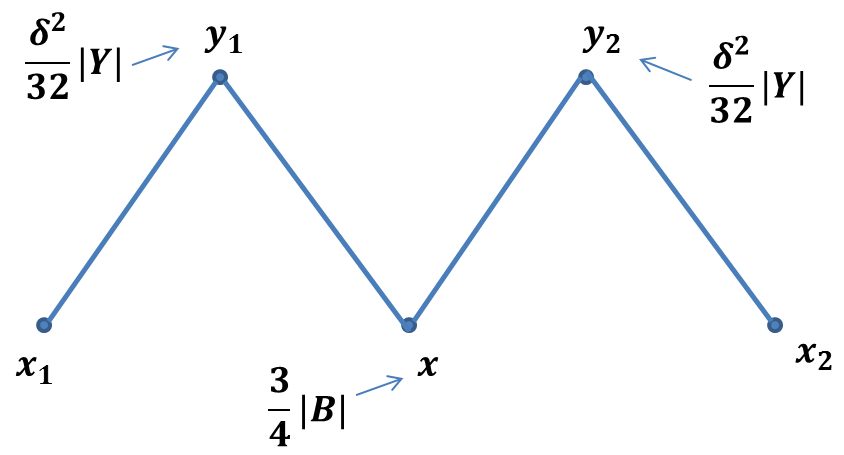
\includegraphics[width=0.3\textwidth]{1}
\end{figure}
Therefore, there at least
\begin{align*}
\frac{\delta^4}{1024} |Y|^2 \frac{3}{4} \frac{\delta |X|}{\sqrt{2}} \quad \text{paths of length 4 from } x_1 \text{ to } x_2
\end{align*} 



[Note : setting $\eta= 1/8$ would(?) give a bound of $\frac{\delta^4}{256} |Y|^2 \frac{1}{2} \frac{\delta |X|}{\sqrt{2}}$]

\eop
\end{proof}
\s

\lemnum{11} \emph{(The BSG Lemma)} Let $A$ be a subset of size $n$ of an Abelian group $H$. Suppose that there are at least $cn^3$ additive quadruples in $A$. Then $A$ has subset $A'$ of size at least $c'n$ with $|A'-A'| \leq C|A'|$, where $c'$ and $C$ depend on $c$ only.
\begin{proof}
\pf For each $d$, let $f(d)$ be the number of ways of writing $d = a_1 -a_2$ with $a_1, a_2 \in A$. Then $\sum_d f(d)^2 \geq cn^3$, because $f(d)^2$ is the number of quadruples $(a_1,a_2, a_3, a_4)$ with $d=a_1 - a_2 = a_3 - a_4$ for each $d$. Call $d$ \textbf{popular} if $f(d)\geq cn/2$. Then
\begin{align*}
cn^3 \leq \sum_d f(d)^2 &= \sum_{d \text{ popular}} f(d)^2 + \sum_{d \text{ unpopular}} f(d)^2 \\
&\leq ( \# \text{ popular d}) \times n^2 + \frac{cn}{2} n^2 \quad (\text{since } \sum_d f(d) = n^2)
\end{align*}
Therefore, the number of popular $d$ is at least $cn/2$.

\quad Now define a graph with vertex set $A$, by joining $a_1$ to $a_2$ if $a_1 -a_2$ (or $a_2 -a_1$) is popular. Each popular difference contributes at least $cn/2$ edges so the average degree of the graph is at least $c^2/4$.

\quad By duplicating the vertex set, create a corresponding bipartite graph $G$. By \textbf{Corollary 10} with $\delta = c^2/4$, we can find a subset $B\subset A$ of size at least $\frac{c^2}{8\sqrt{2}} |A|$ such that for any $a_1,a_2 \in B$ there are at least $\frac{\delta^5}{2048\sqrt{2}} |A|^3$ paths of length 4 from $a_1$ to $a_2$. Each such paths of length 4 gives us at least $(\frac{c}{2}|A|)^4$ ways of writing $a_2 -a_1$ as $b_1 -b_2 + b_3 -b_4 +b_5 -b_6 +b_7 -b_8$ with all $b_i \in A$. So

\begin{align*}
|B-B| \times \frac{\delta^5}{2048 \sqrt{2}} |A|^3 (\frac{c}{2}|A|)^4 \leq |A|^8
\end{align*}
so $|B-B|\leq C'|A| \leq C|B|$

\eop
\end{proof}
\s

\newday

(30th October, Tuesday)
\s

(When revising this course, try to remember the structure of the proofs rather than the exact numbers. The exact number is not very important)

\section*{3. Quasirandom Graphs}

The box norm is an extremely useful tool in studying Quasirandomness.

\subsection*{The box norm}
\newcommand{\boxnorm}[1]{\norms{#1}{\square}}
\quad Let $X$ and $Y$ be finites sets and $f:X\times Y \rightarrow \mathbb{C}$. We define the \textbf{box norm} $\norms{f}{\square}$ of $f$ by the formula
\begin{align*}
\boxnorm{f}^4 = \avg_{x_1,y_1,x_2,y_2} f(x_1,y_1) \bar{f(x_1,y_2)}\bar{f(x_2,y_1)} f(x_2,y_2)
\end{align*}
It is not entirely clear if whether this really is a norm.
\s

\quad If $f_1,f_2,f_3,f_4 :X\times Y \rightarrow \mathbb{C}$, then their \textbf{box inner product} $[f_1,f_2,f_3,f_4]$ is
\begin{align*}
[f_1,f_2,f_3,f_4] = \avg_{x_1,y_1,x_2,y_2} f_1(x_1,y_1) \bar{f_2(x_1,y_2)} \bar{f_3(x_2,y_1)} f_4(x_2,y_2)
\end{align*}
\s

We shall \emph{temporarily} use the notation $[f_1,f_2,f_3,f_4]=\boxinn{f_1}{f_2}{f_3}{f_4}$ in order to expose the symmetry.
\s

\lemnum{1} For any four functions $f_00, f_{01}, f_{10}, f_{11}$ we have
\begin{align*}
|\boxinn{f_{00}}{f_{01}}{f_{10}}{f_{11}}| \leq \boxnorm{f_{00}} \boxnorm{f_{01}}\boxnorm{f_{10}}\boxnorm{f_{1}}
\end{align*}
This is called \textbf{Box Cauchy-Schwarz inequality}.
\begin{proof}
\pf \begin{align*}
& \avg_{x_0,y_0,x_1,y_1} f_{00}(x_0,y_0) \bar{f_{01}(x_0,y_1)} \bar{f_{10}(x_1,y_0)} f_{11}(x_1,y_1) \\
=& \avg_{x_0,x_1} \Big( \avg_{y_0} f_{00}(x_0,y_0)   \bar{f_{10}(x_1,y_0)} \Big) \overline{\Big( \avg_{y_1} f_{01}(x_0,y_1) \bar{f_{11}(x_1,y_1)} \Big)} \\
\leq&  \Big( \avg_{x_0,x_1} \Big| \avg_{y_0} f_{00}(x_0,y_0) \bar{f_{10}(x_1,y_0)} \Big|^2 \Big)^{1/2} \Big( \avg_{x_0,x_1} \Big| \avg_{y_1} f_{01}(x_0,y_1) \bar{f_{11}(x_1,y_1)} \Big|^2 \Big)^{1/2} \\
=& \boxinn{f_{00}}{f_{00}}{f_{10}}{f_{10}}^{1/2} \boxinn{f_{01}}{f_{01}}{f_{11}}{f_{11}}^{1/2}
\end{align*}
By Symmetry (interchanging the roles of $x$ and $y$) we also have, for any functions $g_{00}, g_{01}, g_{10}, g_{11}$, 
\begin{align*}
\Big| \boxinn{g_{00}}{g_{01}}{g_{10}}{g_{11}} \Big| \leq \boxinn{g_{00}}{g_{01}}{g_{00}}{g_{01}}^{1/2} \boxinn{g_{10}}{g_{11}}{g_{10}}{g_{11}}^{1/2}
\end{align*}
Combining these two inequalities in the obvious way gives the result.

\eop
\end{proof}
(the whole point of using this weird notation was to visualize symmetry and to simplify the argument. Can give up with this notation and write a lengthy proof)
\s

\cornum{2} $\boxnorm{\cdot}$ is a norm.
\begin{proof}
\pf The only property that is not completely straightforward is the triangular inequality. Let $f_0$, $f_1: X\times Y \rightarrow \mathbb{C}$. Then
\begin{align*}
\boxnorm{f_0 + f_1}^4 &=  [f_0+f_1 ,f_0+f_1,f_0+f_1,f_0+f_1] \\
&= \sum_{\epsilon \in \{0,1\}^4} [f_{\epsilon_1},f_{\epsilon_2},f_{\epsilon_3},f_{\epsilon_4}] \\
&\leq \sum_{\epsilon \in \{0,1\}^4} \boxnorm{f_{\epsilon_1}} \boxnorm{f_{\epsilon_2}} \boxnorm{f_{\epsilon_3}} \boxnorm{f_{\epsilon_4}} \\
&= (\boxnorm{f_0} + \boxnorm{f_1})^4
\end{align*}

\eop
\end{proof}
\s

\textbf{Remark :} Suppose that $f(x,y) = g(x)$ for every $x,y$. Then
\begin{align*}
\boxnorm{f}^4 = \avg_{x_1,x_2} g(x_1) \bar{g(x_1)} \bar{g(x_2)} g(x_2) = \norms{g}{2}^4
\end{align*}
so $\boxnorm{f} = \norms{g}{2}$.
\s

\cornum{3} \emph{(The box-norm inequality)} If $f: X \times Y \rightarrow \mathbb{C}$, $u:X\rightarrow \mathbb{C}$, $v:Y\rightarrow \mathbb{C}$ then
\begin{align*}
\big| \avg_{x,y} f(x,y) u(x) v(y) \big| \leq \boxnorm{f} \norms{u}{2} \norms{v}{2}
\end{align*}
\begin{proof}
\pf Apply the box Cauchy-Schwarz inequality to $f_1=f$, $f_2(x,y) = u(x)$, $f_3(x,y) =v(y)$, $f_4(x,y)=1$ and use the above remark.

\eop
\end{proof}
\s

\lemnum{4} Let $f: X\times Y \rightarrow \mathbb{C}$. Then $\boxnorm{f} \geq |\avg_{x,y} f(x,y)|$.
\begin{proof}
\pf Note that we can write $\boxnorm{f}^4 = \avg_{x_1,x_2}  \big| \avg_y f(x_1,y) \bar{f(x_2,y)} \big| ^2$, so
\begin{align*}
\boxnorm{f}^4 &= \avg_{x_1,x_2}  \big| \avg_y f(x_1,y) \bar{f(x_2,y)} \big| ^2 \geq \big| \avg_{x_1,x_2} \avg_y f(x_1,y) \bar{f(x_2,y)} \big|^2 \\
&= \Big| \avg_y \big| \avg_x f(x,y) \big|^2 \Big|^2 \geq \Big| \avg_y \avg_x f(x,y)   \Big|^4
\end{align*}

\eop
\end{proof}
\s

\lemnum{5} Let $F: X\times Y \rightarrow \reals$ be such that $\avg_{x,y} F(x,y) = \delta >0$ and $\boxnorm{F} \leq \delta^4 (1+C)$. Let $f(x,y) = F(x,y) - \delta$. Then $\boxnorm{f} \leq $.
\s

\quad This inequality can be thought to be an estimation of box norm-variance of $F$.
\begin{proof}
\pf For each $x$, let $g(x) = \avg_{y} f(x,y)$ and let $h(x,y)= f(x,y) - g(x)$. Then $\avg_x g(x) = \avg_{x,y} f(x,y) = \avg_{x,y} F(x,y) - \delta =0$ and for every $x$, $\avg_{y} h(x,y) = g(x) - g(x) = 0$. Now 
\begin{align*}
\boxnorm{F}^4 &= \avg_{x_1,x_2}  \big| \avg_y F(x_1,y) \bar{F(x_2,y)} \big| ^2 \\
&= \avg_{x_1,x_2} \Big| \avg_y (\delta + g(x_1) + h(x_1,y))(\delta + \bar{g(x_2)} + \bar{h(x_2,y)})\Big|^2 \\
&= \avg_{x_1,x_2} \Big| \avg_y (\delta + g(x_1))(\delta + \bar{g(x_2)}) + \avg_y h(x_1,y) \bar{h(x_2,y)} \Big|^2 \\
&\geq \delta^4 + 2\delta^2 \avg_x |g(x)|^2 + (\avg_x |g(x)|^2)^2 + \boxnorm{h}^4
\end{align*}

(...to be continued)
\end{proof}


















\end{document}